\begin{frame}{USB - Bus Serial Universal}
	\centering
	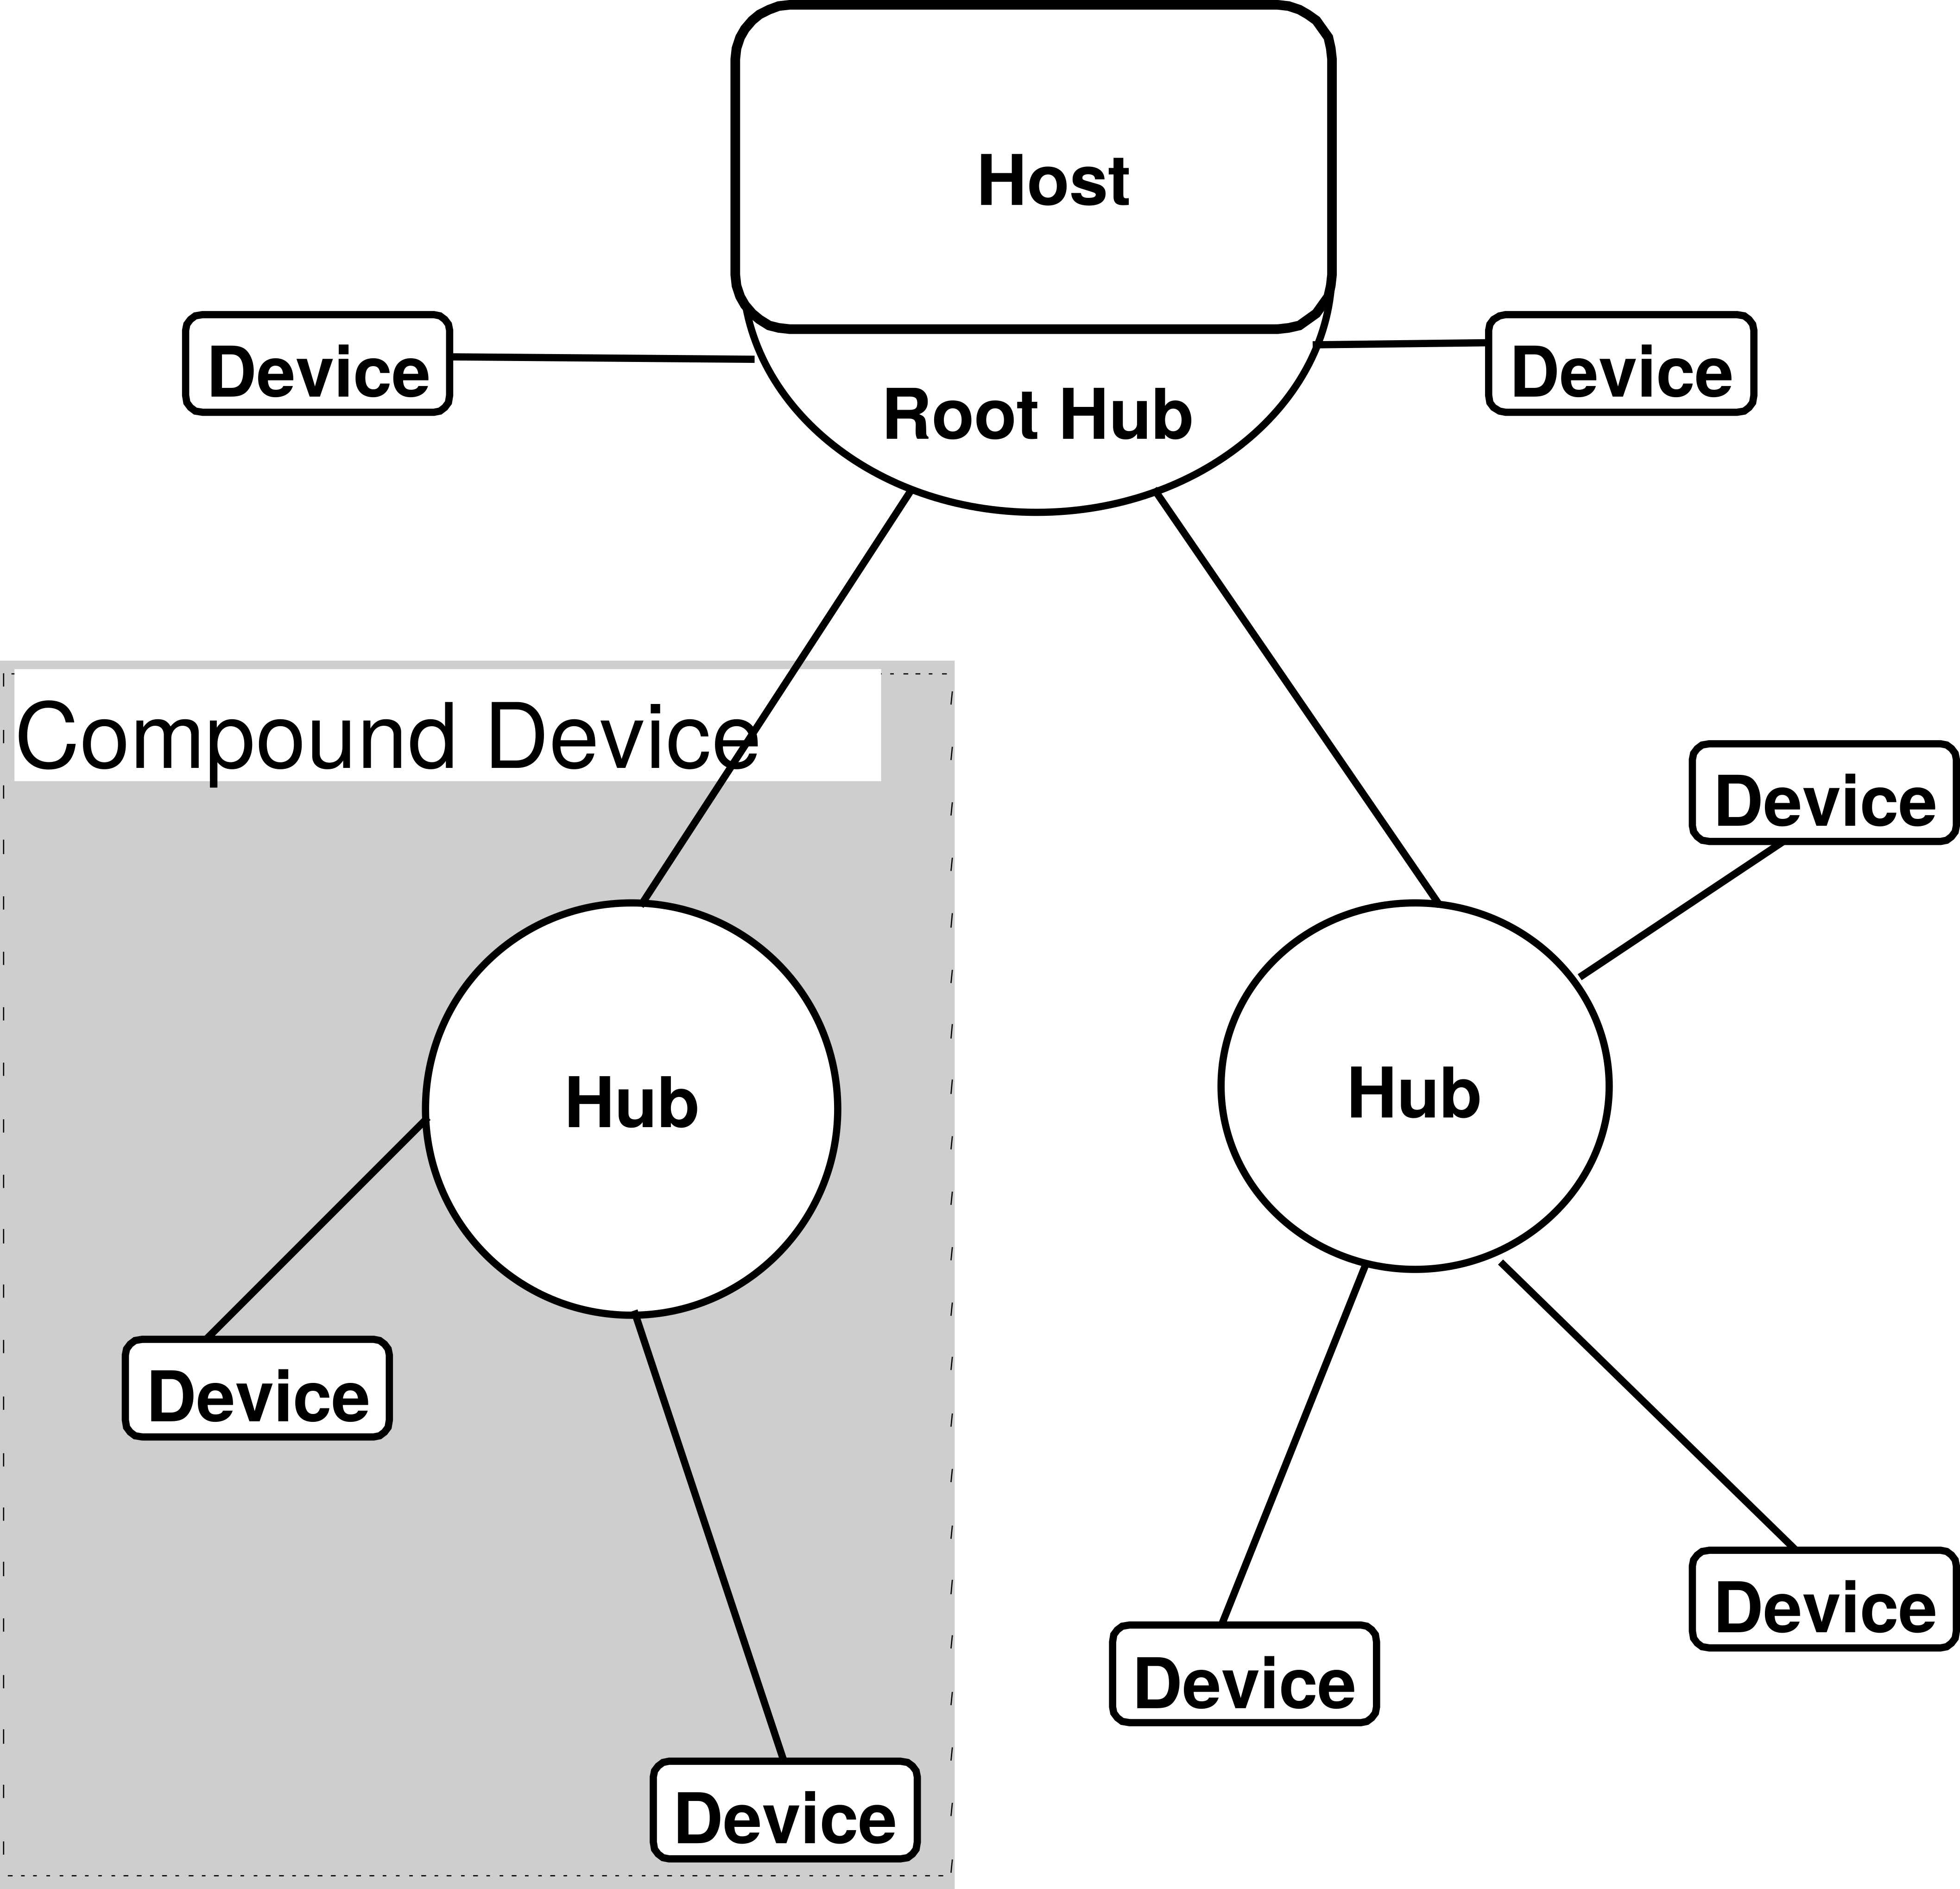
\includegraphics[width=0.6\textwidth]{topofisica.png}
	\blfootnote{Compaq, Hewlett-Packard, Intel, Lucent, Microsoft, NEC and Philips, \textit{Universal Serial Bus Specification}, Revision 2.0. }
\end{frame}


\begin{frame}{USB 2.0 - Velocidades de operación}
	\centering
	\begin{columns}
		\begin{column}{.3\textwidth}
			
\includegraphics[width=\columnwidth]{usb10}
		\end{column}
		\begin{column}{.6\textwidth}
			\huge{Low-Speed: 1.5 Mbps} 
		\end{column}
	\end{columns}
	\hfill
	\begin{columns}
		\begin{column}{.3\textwidth}
			
\includegraphics[width=\columnwidth]{usb11}
		\end{column}
		\begin{column}{.6\textwidth}
			\huge{Full-Speed: 12 Mbps} 
		\end{column}
	\end{columns}
	\hfill
	\begin{columns}
		\begin{column}{.3\textwidth}
			
\includegraphics[width=\columnwidth]{usb20}
		\end{column}
		\begin{column}{.6\textwidth}
			\huge{High-Speed: 480 Mbps} 
		\end{column}
	\end{columns}	
	\blfootnote{Compaq, Hewlett-Packard, Intel, Lucent, Microsoft, NEC and Philips, \textit{Universal Serial Bus Specification}, Revision 2.0. }
\end{frame}

\begin{frame}{USB - Tipo de transferencias}
	\centering
	\begin{itemize}
		\item Control: Destinada a comunicaciones de control y estado del bus entre el Host y los Dispositivos.
		\item Interrupción: Posee latencia mínima. Destinada a comunicaciones no periódicas.
		\item \alert<2>{Isócronas:} Acceso periódico al bus. Sin retransmisión de mensajes. Destinada a la comunicación que caduca con demoras en la entrega, como imágenes.
		\item \alert<3>{en Masa:} Destinada a maximizar la ocupación del bus.
	\end{itemize}
	\vspace{1.5em}
	\begin{tikzpicture}[scale=1]
		\centering
		\begin{scope}[node distance=2]
			\action<2-3>{\node[exterior,rounded corners](pc){PC};}
			\action<2-3>{\node[exterior,rounded corners](fpga)[right=of pc]{FPGA};}
			\only<2>{\draw[blue,ultra thick,<-](pc)to(fpga);}
			\only<3>{\draw[blue,ultra thick,->](pc)to(fpga);}
		\end{scope}
	\end{tikzpicture}
	\blfootnote{Compaq, Hewlett-Packard, Intel, Lucent, Microsoft, NEC and Philips, \textit{Universal Serial Bus Specification}, Revision 2.0. }
\end{frame}
